\subsection{Padded Blocks}
Consider a loop of the following form:
\begin{verbatim}
for (int i = 0; i < I; ++i) {
  for (int j = 0; j < J; ++j) {
    do_stuff(i, j);
  }
}
\end{verbatim}
When \ttt{I} and \ttt{J} are values that are unknown at compile time, the
compiler is limited in the optimizations it can perform. For example, if it
unrolls the loop, it must be careful that the unroll factor divides \ttt{I} or
\ttt{J}. If it does not, then it has to perform some of the computation in the
unrolled loop and insert remainder loops to perform the remaining computation.

When \ttt{I} and \ttt{J} are known at compile time, the compiler can perform
additional optimizations. For example, it can perform more educated loop
unrolling and can more efficiently use vector instructions.

The \ttt{padded\_blocked} kernel uses copy optimization and padding in such a
way that our inner most loops have bounds known at compile time. Concretely,
the \ttt{padded\_blocked} kernel defines a compile time constant \ttt{BLOCK\_SIZE}.
The kernel performs a blocked matrix multiplication where a block $A_{ik}$ of
$A$ is multiplied by a block $B_{kj}$ of $B$ to produce a block $C_{ij}$ of
$C$. Before each block multiplication, $A_{ik}$ is copied into a buffer of size
$\ttt{BLOCK\_SIZE} \times \ttt{BLOCK\_SIZE}$ in row-major order. Similarly
$B_{kj}$ is copied into a buffer of the same size in column-major order. If
ether $A_{ik}$ or $B_{kj}$ is smaller than the buffer, then the remaining
elements are zeroed.

We performed a parametric sweep on the block size of the \ttt{padded\_blocked}
kernel to decide on an optimal block size. The results of the sweep can be
found in \figref{padded-sweep}. A block size of 128 was selected.

\begin{figure}[h]
  \centering
  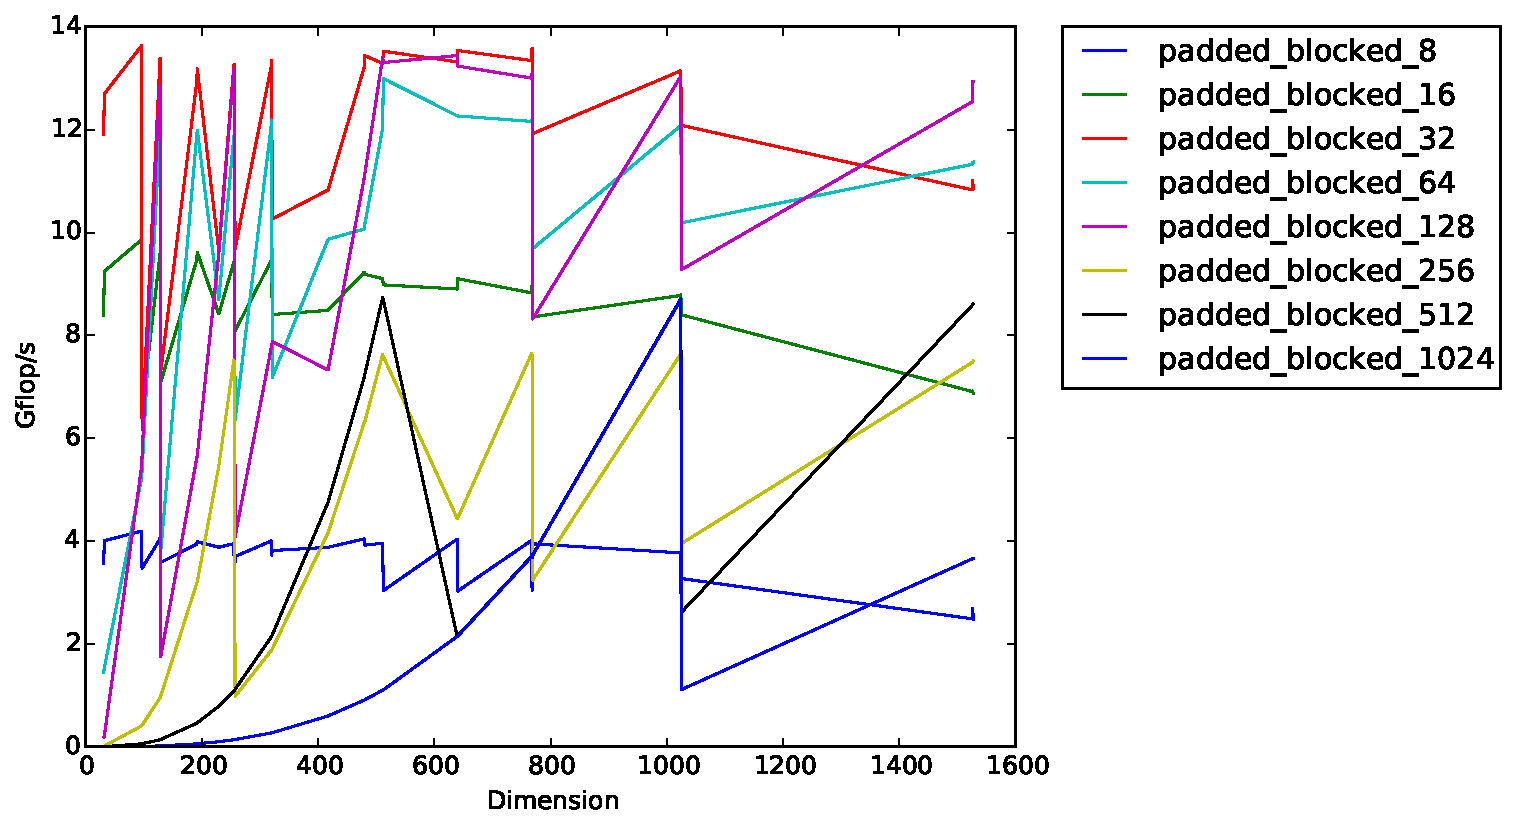
\includegraphics[width=\textwidth]{img/timing_padded_sweep.pdf}
  \caption{Parametric sweep of block size for the \ttt{padded\_blocked} kernel.}
  \label{fig:padded-sweep}
\end{figure}
